
\chapter{Two-Dimensional SEAS model}
In a second step we consider a trivial SEAS model with only two dimensions and square, symmetric tectonic plates.

\section{Physical Description}
\label{ssec:physicalDescriptionSEAS2D}
--- write down Poisson/elasticity equation for the domain --- \\
--- rate and state laws for the fault --- \\
describe what all variables mean and stuff...
Ageing law: 
\begin{equation}
    \dot{\psi} = g(\psi, V) = \frac{bV_0}{L}e^{\frac{f_0 - \psi}{b}} - \frac{V}{V_0}
\end{equation}
Friction law: 
\begin{equation}
    0 = \tau(U) - a\sigma_n(U) \text{arsinh}\left(\frac{V}{2V_0}e^{\frac{\psi}{a}}\right) - \eta V
\end{equation}


\section{BP1 problem}
--- read more about BP1 and find good citations --- \\
The displacement is applied orthogonal to the represented plane, thus, if the mesh is located in the X-Y plane, each element has one traction, velocity and displacement component acting in the Z direction. In this model problem, the represented tectonic plates have a symmetric layout and move in opposite direction, as one moves into the plane and the other one out of the plane. Therefore, it is enough to consider only one half of the domain, as the results in the other half will be identical, but with opposite sign. \autoref{fig:mesh_BP1_200_fault_elements} depicts the half-domain on which the solution is calculated. The fault is located on the left side of the domain.
\begin{figure}[H]
    \centering
    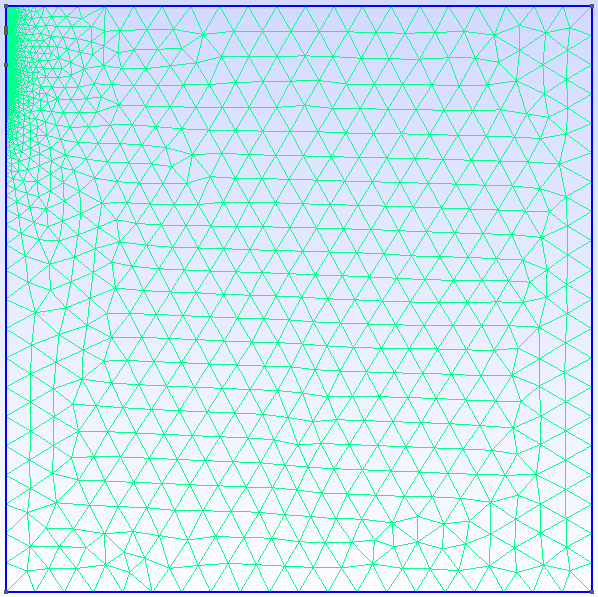
\includegraphics[width=0.4\textwidth]{images/BP1_MESH_200.png}
    \caption{Space discretization of the BP1 problem with 200 elements on the fault}
    \label{fig:mesh_BP1_200_fault_elements}
\end{figure}

In the considered example, we choose the mesh such that there are 200 elements at the fault. The lower end of the plates is pulled with a constant velocity $V_0 = 10^{-6} m\cdot s^{-1}$. 

\section{Formulation of the Discontinous Galerkin}

--- write something about DG --- \\ 


The numerical integration is achieved with the Gaussian quadrature. For that, Gauss-Legendre polynomials up to order $p$ are chosen to interpolate relevant values on each element. Dependent on the chosen order $p$, the solution has to be calculated at different points $x_i$ within the element and, associated with the correct weights to interpolate the data over the entire element, the integration is exact with respect to the interpolation polynomials. \\
--- write more about GQ --- \\

To solve the Poisson equation, it is necessary to evaluate the integral over the entire element and to handle boundary conditions and the fault, the integral over the edges of the element is needed. 

\section{Evolution of Quantities}
\begin{figure}[H]
	\centering
	\includegraphics[width=0.7\textwidth{images/TANDEMtimeEvolution_MinMaxAllStacked_Size200_RKDP5_extendedODE}
	\label{fig:EvolutionAllQuantitiesMinMaxStacked200Elements}
	\caption{Evolution of the slip $S$, the state variable $\psi$ and the slip rate $V$ over 770 years on a domain with 200 fault elements}
\end{figure}
